\ssection{BASIC CONCEPTS ON CARDIAC ANATOMY AND ELECTROPHYSIOLOGY} \label{Some_Basis_on_Anatomy_and_Electrophysiology}

The heart is a double pump consisting of four chambers, two atria in the upper part, separated by the inter-atrial septum and two ventricles in the lower part, separated by the inter-ventricular septum. See Figure \ref{corazon} for a hearth scheme and \cite{electrofis} for more details. 

\begin{figure}[!htbp] % esquema corazón
\centering
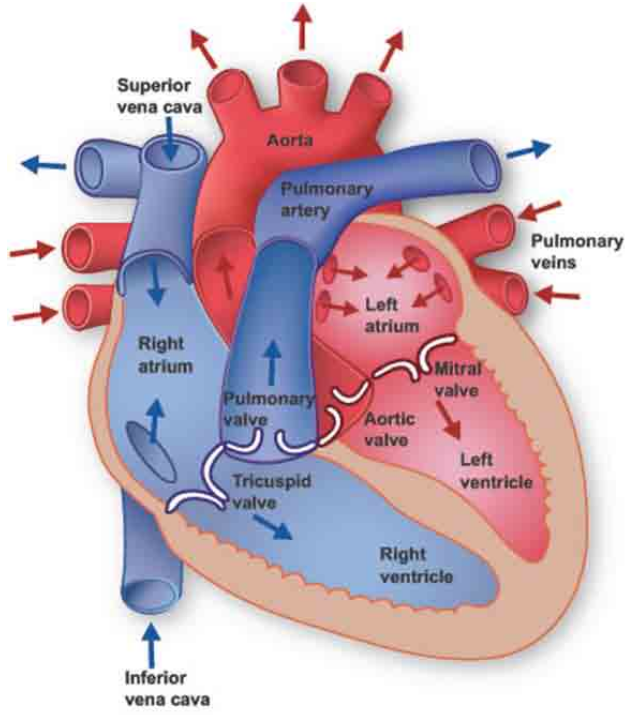
\includegraphics[height = 6 cm]{fig/fundamentals-corazon}
\caption{Schematic diagram of the heart anatomy.} \label{corazon}
\end{figure}

The electric potential wave genesis responsible of the cardiac muscle cells contraction occurs due to an autonomous depolarization in the sinoatrial node (SAN), located at the upper part of right atria. Then, the wave propagation is achieved because this depolarization changes the membrane potential of surrounding cardiac cells (due,  actually, to a cellular membrane ionic flow). The potential wavefronts travel first in the right atria, then into the left one. Next, the atrio-ventricular node (AVN) is reached, which conveniently has a high electric resistivity, in order to generate a control delay in the propagation, preventing any early ventricular stimulation. Finally, the Purkinge network (see Figure \ref{corazon_conduccion}) enable a fast potential propagation to ventricles chamber.

\begin{figure}[!htbp]% esquema conducción de corriente en el corazón
\centering
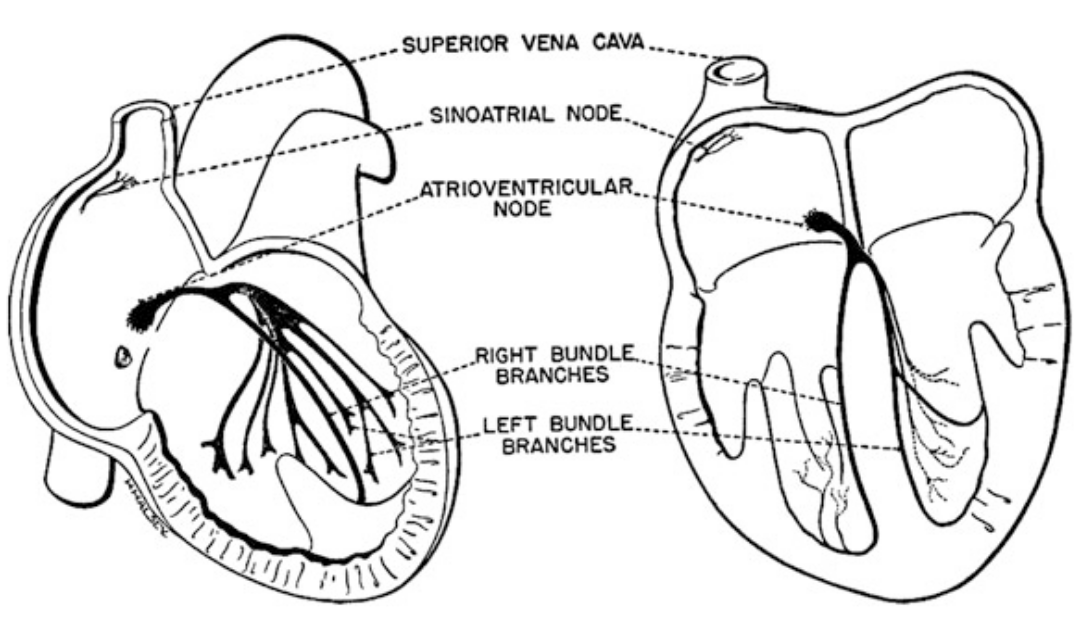
\includegraphics[height = 6 cm]{fig/fundamentals-sistema_de_conduccion}
\caption{Schematic diagram of the heart conduction system.} \label{corazon_conduccion}
\end{figure}

\subsection{Cardiac Tissue Organization} \label{Cardiac_Tissue_Organization}

The contract/relax macroscopic behavior of the heart is achieved due to collective cell activity. This cells, called myocites, works together joint by \textsl{gap junctions} which allows a quick electrical propagation in a particular direction, often called \textsl{the fiber direction}. Each one of this myocites has internal protein arrays called myofibrils, as can be seen in Figure \ref{fig:myocite}, which enables most part of the elastic properties of cardiac tissue.

Also, in the cardiac tissue exist another type of cells called \textsl{fibroblasts}, who are responsible of synthesize the extracellular matrix (ECM), an extensive and highly organized network of fibrous proteins, elastic and collagen (the main structural protein of the extra-cellular space in the human and other animals connective tissue). Specifically, the proportion of this last protein over the remain tissue can be used to measure fibrosis intensity.

\begin{figure}[!htbp]
	\centering
	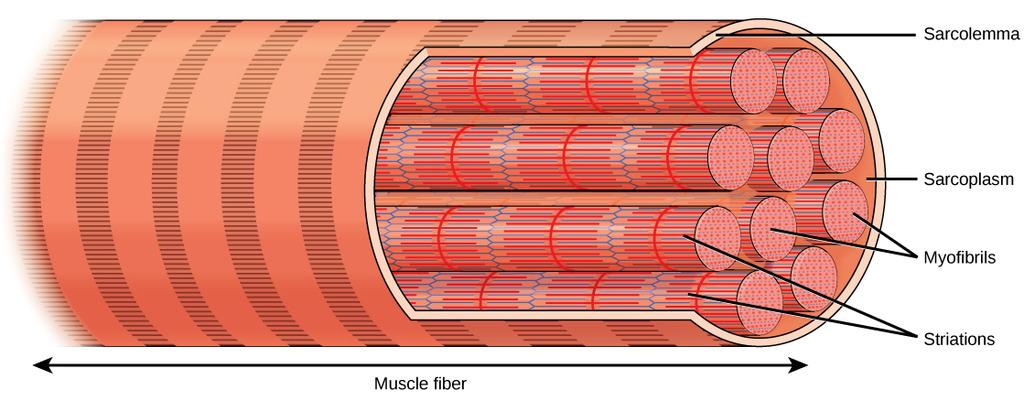
\includegraphics[height = 4 cm]{fig/fundamentals-myocites}
    \caption{Schematic view of a myocite.} 
    \label{fig:myocite}
\end{figure}

\begin{figure}[!htbp]
	\centering
    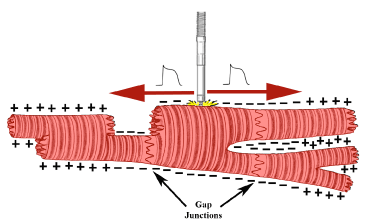
\includegraphics[height = 5 cm]{fig/fundamentals-gap_junctions} 
    \caption{Gap junctions: sarcoplasm electrical bypass of the myocites.}
    \label{fig:gap_junctions}
\end{figure}


Myocites and the ECM are arranged together within a complex three-dimensional spatial organization, with a fiber and laminar structure, like in Figure \ref{orientacionmiocitos}. This organization, as can be expected, affects the diffusion properties of the tissue, which is consequently highly anisotropic. This last usually is represented by a second-rank tensor, that can be written as a $3 \times 3$ matrix. The three orthogonal eigenvector of this tensor can be related directly to cardiac structure. In fact, the primary eigenvector (i.e. the eigenvector with largest eigenvalue) relays in the fiber long axis direction, the secondary eigenvector relays orthogonal to fiber long axis direction (cross-fiber direction), in the myolaminar plane, while the minor eigenvector, orthogonal to both fiber and cross-fiber directions, will be normal to the myolaminar plane.

\subsection{Action Potential} 

As established above, cardiac cells are excitable, some autonomously and some others after a proper electrical stimulus. The excitation of a cardiac cell causes a rapid variation of its potential difference across the cell membrane, the so-called \textsl{transmembrane potential}. There exist a minimum value of potential difference stimulus below the cell will react, a threshold, that if is reached, the cell membrane depolarizes and the trans-membrane potential changes from a resting negative value to a slightly positive one. This complete event is called an \textsl{action potential}, and phases can be identified, according to the activation of different membrane ionic channels. One action potential cycle can be seen in Figure \ref{action-potential}. 

\begin{figure}[!htbp]
\centering
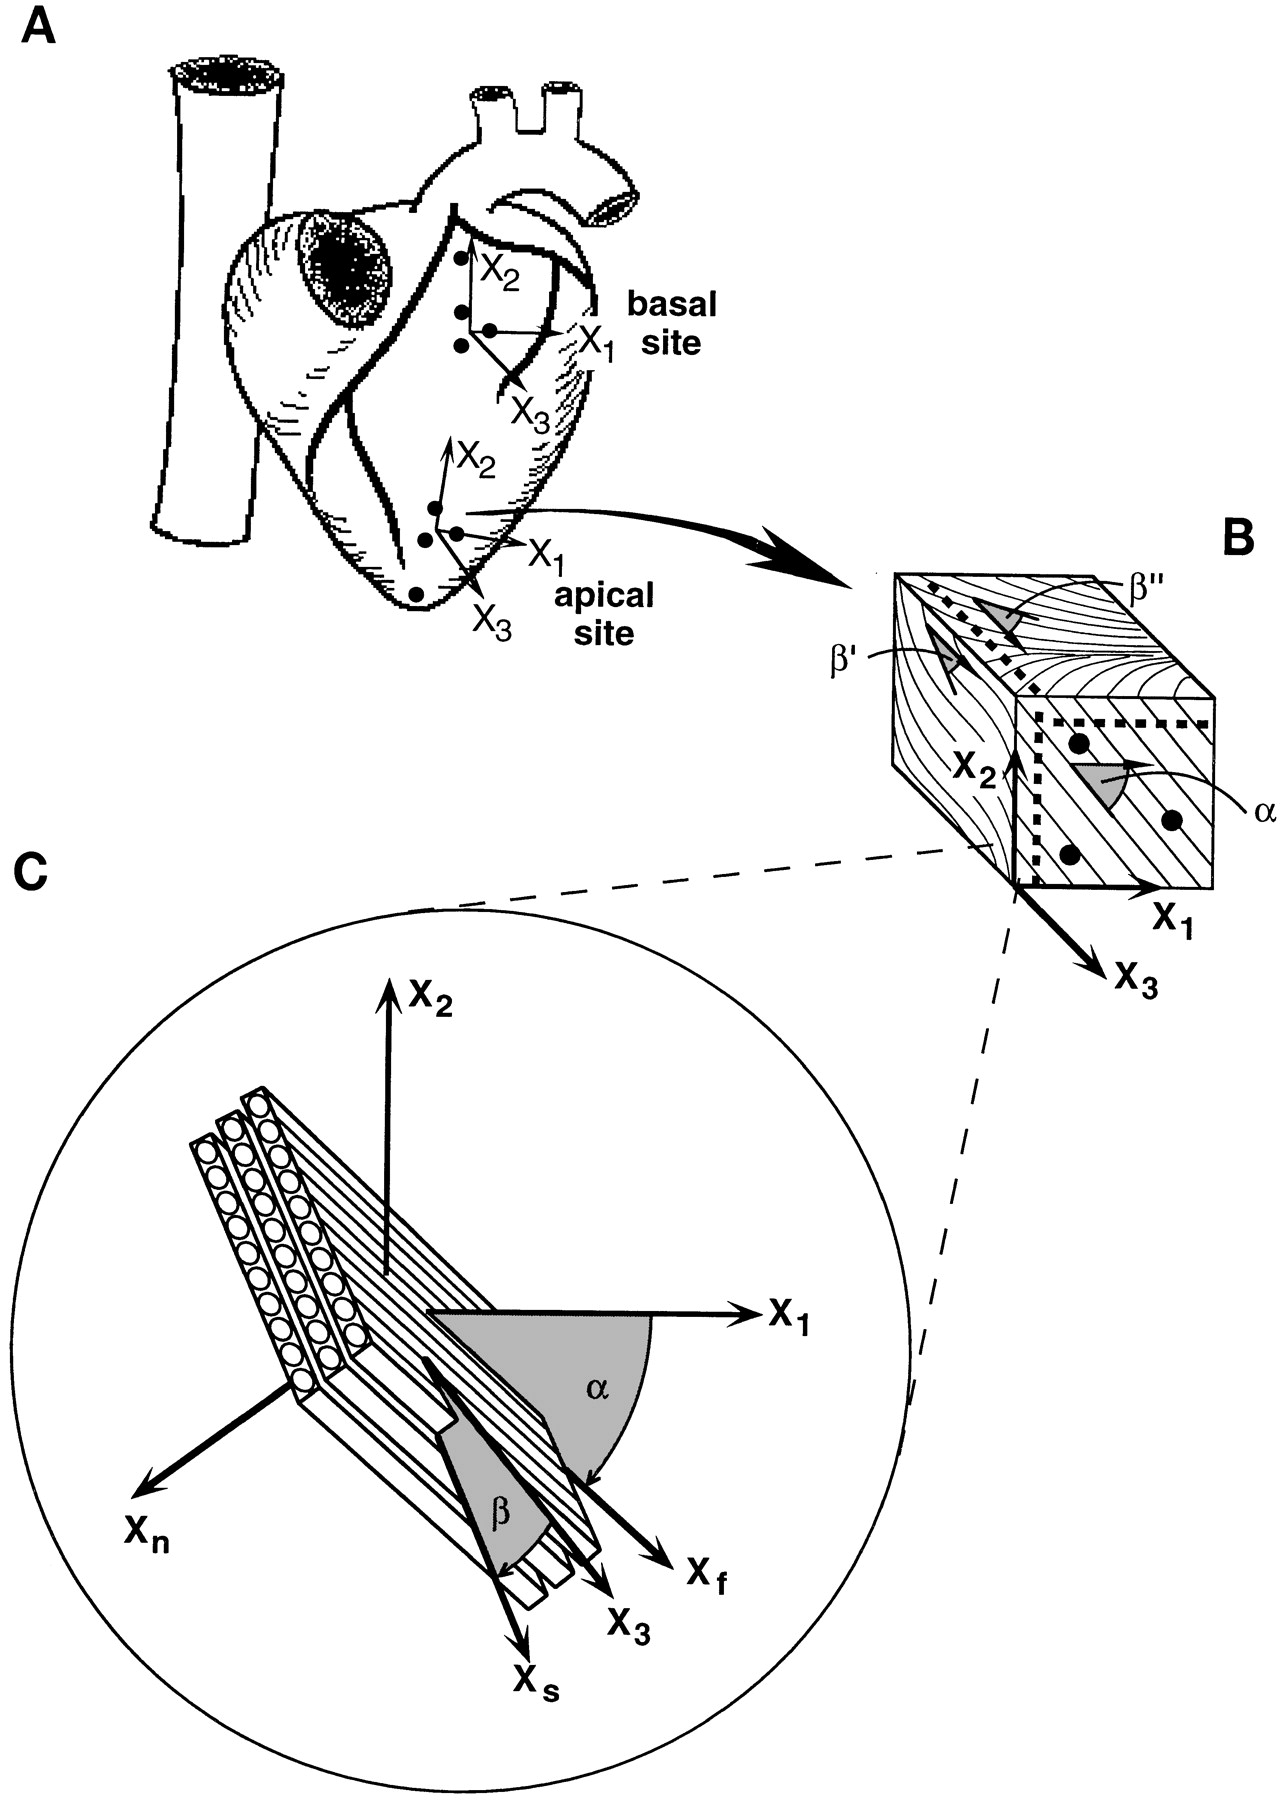
\includegraphics[scale=.14]{fig/fundamentals-direccionmiocitos}
\caption{Heart fiber orientation.} \label{orientacionmiocitos}
\end{figure}

The extracellular potential can be registered in a electrocardiogram (ECG), which can eventually lead us to diagnose some diseases as consequence of fibrosis, as the sinus bradycardia and tachycardia, arrhythmias, paroxysmal atrial tachycardia, etc.

\begin{figure}[!htbp]
\centering
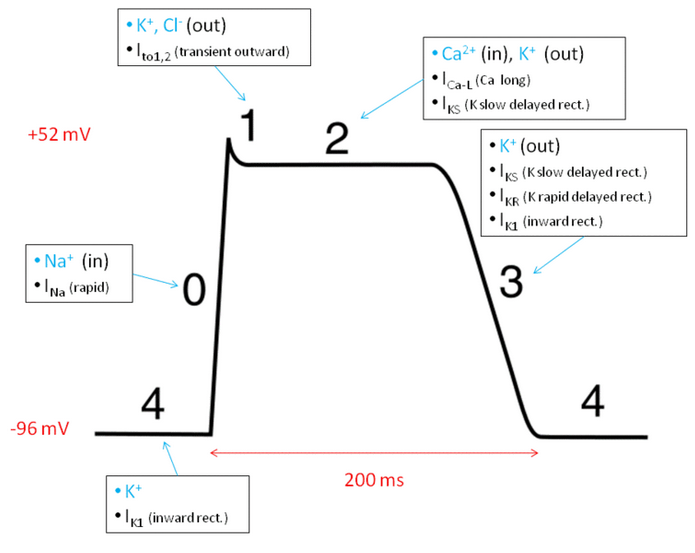
\includegraphics[height = 7 cm]{fig/fundamentals-action_potential}
\caption{Schematic plot of a cardiac action potential with its phases.} \label{action-potential}
\end{figure}

\subsection{Fibrosis} \label{Fibrosis}

Cardiac fibrosis is the excess of fibrous connective tissue, mostly collagen, as consequence of a self-regenerative process done by the fibroblasts. 

Different patterns of fibrosis has been observed accordingly to extra connective tissue percentage (density or intensity of fibrosis) and the dispersion of fibrotic areas in the tissue, i.e., the fibrosis architecture. Furthermore, according to this two statistical parameters, three types of fibrosis can be distinguished \cite{Kawara2001Circ}: \textsl{stringy}, \textsl{diffuse} and \textsl{patchy}. The stringy fibrosis architecture is characterized by homogeneously distributed collagen laminations with long and single strands. In patchy patterns arise long and compact groups of strands. Finally, diffuse fibrosis pattern is characterized with more or less homogeneously distributed small collagen short strands. The Figure \ref{fig:fibrosis_typology} shows the different types of fibrosis

The remarkable thing is that some studies \cite{Comtois2011IEEE} suggest that when a density threshold is reached, only spatial distribution of connective tissue affects the electric potential propagation velocity. In a recent research \cite{Kawara2001Circ}, the mean increase of the propagation delay (MID) was measured for failed human hearts with different fibrosis intensities. A result of this study can be seen in Figure \ref{fig:midvsdensity}, where the spatial distribution dependency of the parameter can be appreciated. Note that high values of MID are usually associated with patchy or stringy fibrosis. On the other hand, areas with diffuse fibrosis, low values of MID are found, even at high densities of fibrosis.

\begin{figure}[!htb]
\centering
\subfigure[Stringy Fibrosis.]{
    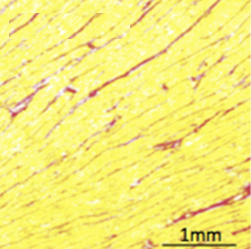
\includegraphics[height = 5 cm]{fig/fundamentals-fib-stringy}
    \label{fig:stringy}
}
\subfigure[Patchy Fibrosis. ]{
    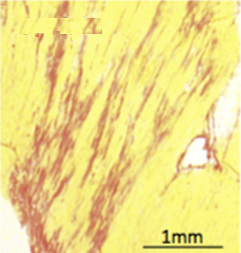
\includegraphics[height = 5 cm]{fig/fundamentals-fib-patchy} 
    \label{fig:patchy}
}
\subfigure[Diffuse Fibrosis. ]{
    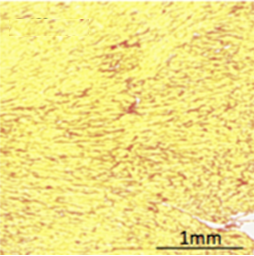
\includegraphics[height = 5 cm]{fig/fundamentals-fib-diffuse} 
    \label{fig:diffuse}
}
\caption{Different types of fibrosis.} \label{fig:fibrosis_typology}
\end{figure}



\begin{figure}[!htb]
	\centering
	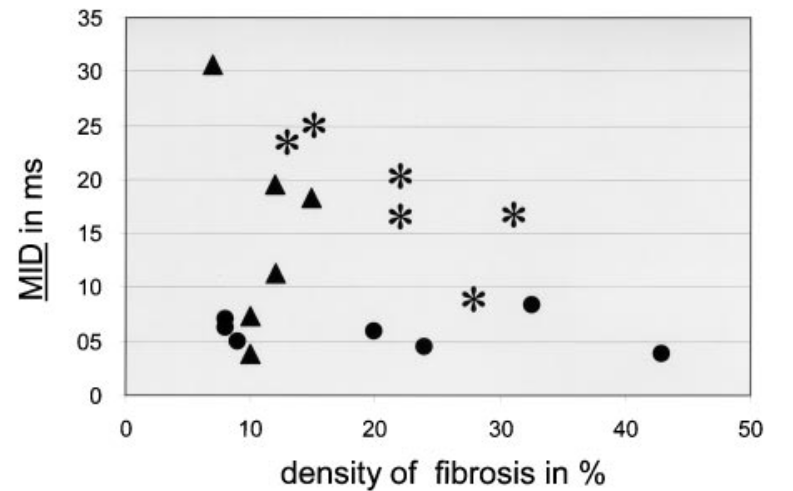
\includegraphics[height = 5 cm]{fig/fundamentals-fib-midvsdensity}
	\caption{Scatterplot of density of fibrosis and MID for different types of fibrosis (patchy, $*$; stringy, $\blacktriangle$; or diffuse, $\bullet$)}. \label{fig:midvsdensity}
\end{figure}
